\documentclass[12pt]{article}

\usepackage{sbc-template}
\usepackage[utf8]{inputenc}
\usepackage[T1]{fontenc}
\usepackage[english]{babel}

\usepackage{graphicx,url}
\usepackage{amsmath,amssymb}
\usepackage{booktabs}
\usepackage{multirow}
\usepackage{float}
\usepackage[hidelinks]{hyperref}

\newcommand{\citep}{\cite}
\newcommand{\citet}{\cite}

% ------------------------------------------------------------------
% Clean STIL/SBC template for the new paper.
% Current fixed information:
% - Authors: Joao Victor M. Correa and Renato Moraes Silva
% - Institution: NILC / ICMC / USP
% - Main bibliography file: bib/bib_main.bib
% - Suggested figures folder: figs/
%
% Replace the placeholders below as the paper evolves.
% Keep the commented examples at the end of the file for quick reuse.
% ------------------------------------------------------------------

\title{Working Title of the Paper}

\author{
Jo\~ao Victor M. Corr\^ea\inst{1}
\and
Renato Moraes Silva\inst{1}
}

\address{
Interinstitutional Center for Computational Linguistics (NILC)\\
Institute of Mathematics and Computer Science\\
University of S\~ao Paulo (USP), S\~ao Carlos, SP, Brazil\\
\texttt{\footnotesize victormcorrea@usp.br, renatoms@icmc.usp.br}
}

\begin{document}

\maketitle

\begin{abstract}
Replace this abstract with a concise summary of the final paper.
For STIL, this usually means five parts in one short paragraph:
the problem, the Portuguese corpus or dataset, the method,
the main empirical result, and the contribution to Portuguese NLP.
\end{abstract}

\section{Introduction}
\label{sec:introduction}

Use this section to explain:
\begin{itemize}
    \item the research problem and why it matters;
    \item why the topic is relevant for Portuguese;
    \item the main gap in prior work;
    \item the paper's research questions or objectives;
    \item the main contribution in one short paragraph.
\end{itemize}

If useful, end the introduction with a short roadmap of the paper.

\section{Related Work}
\label{sec:related_work}

Organize the literature review around the themes that matter for the final paper.
For example:
\begin{itemize}
    \item prior work on semantic change or concept drift;
    \item prior work on Portuguese corpora or Portuguese NLP;
    \item datasets, benchmarks, and methodological gaps.
\end{itemize}

\section{Corpus and Experimental Setup}
\label{sec:data_setup}

Describe the dataset or corpus here.
This section will likely include:
\begin{itemize}
    \item source and collection procedure;
    \item temporal coverage;
    \item filtering and preprocessing;
    \item descriptive statistics;
    \item train, validation, and test split strategy if applicable.
\end{itemize}

\section{Methodology}
\label{sec:methodology}

Explain the analytical pipeline clearly enough that it can be reproduced.
Typical subsections might include:
\begin{itemize}
    \item text representation or embeddings;
    \item temporal aggregation strategy;
    \item drift or semantic change metrics;
    \item baselines and comparison settings;
    \item evaluation criteria.
\end{itemize}

\section{Results and Discussion}
\label{sec:results}

This section should present the main findings and their interpretation.
It often helps to separate:
\begin{itemize}
    \item core quantitative results;
    \item qualitative examples or case studies;
    \item ablations, robustness checks, or comparisons;
    \item implications for Portuguese NLP.
\end{itemize}

\section{Conclusion}
\label{sec:conclusion}

Close with:
\begin{itemize}
    \item the main answer to the research question;
    \item the most important empirical takeaway;
    \item the main limitation;
    \item one or two realistic next steps.
\end{itemize}

\section*{Acknowledgments}

Add funding, institutional support, project grants, or collaboration acknowledgments here.
If the paper is submitted without acknowledgments at first, this section can remain commented out until the final version.

\bibliographystyle{sbc}
\bibliography{bib/bib_main}

% ------------------------------------------------------------------
% Quick examples for reuse
% ------------------------------------------------------------------
% Recommendation:
% - Prefer PDF for plots, charts, line art, and vector graphics.
% - Prefer PNG for screenshots or raster images.
% - Avoid JPG unless the source is a photo and you really need it.
% The files below show both PDF and PNG usage with real assets in figs/archive/.

% Example of citation usage:
% Prior work on semantic change in Portuguese remains limited
% \citep{example_semantic_change_2024}.
% \citet{example_dataset_2023} provides a useful Portuguese corpus.

% Example of a single image / figure:
% \begin{figure}[H]
%     \centering
%     % Prefer PDF here because this is a vector plot.
%     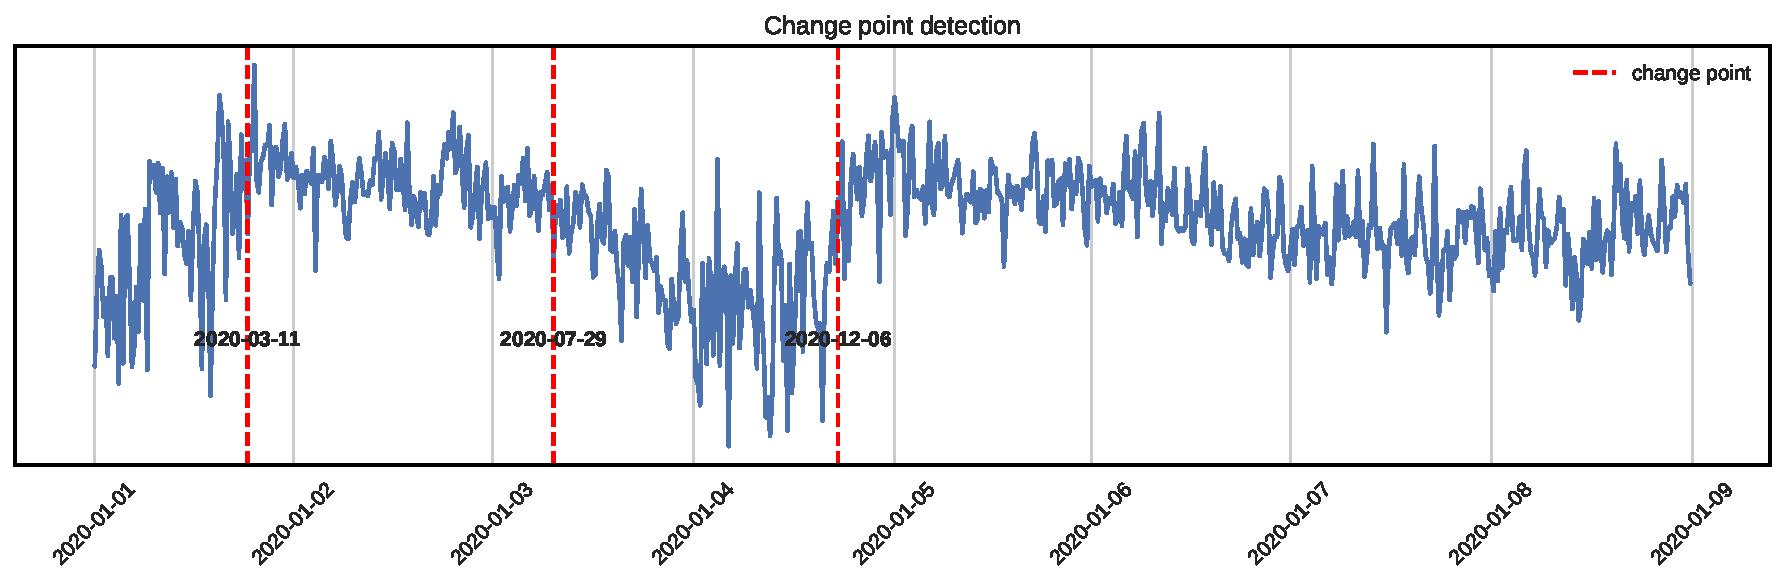
\includegraphics[width=0.8\linewidth]{figs/archive/change_point_detection.pdf}
%     \caption{Example using a PDF figure from the figs/ folder.}
%     \label{fig:cpd_example}
% \end{figure}

% Example of two images side by side:
% \begin{figure}[H]
%     \centering
%     \begin{minipage}{0.48\linewidth}
%         \centering
%         % PDF is preferred for plots and charts.
%         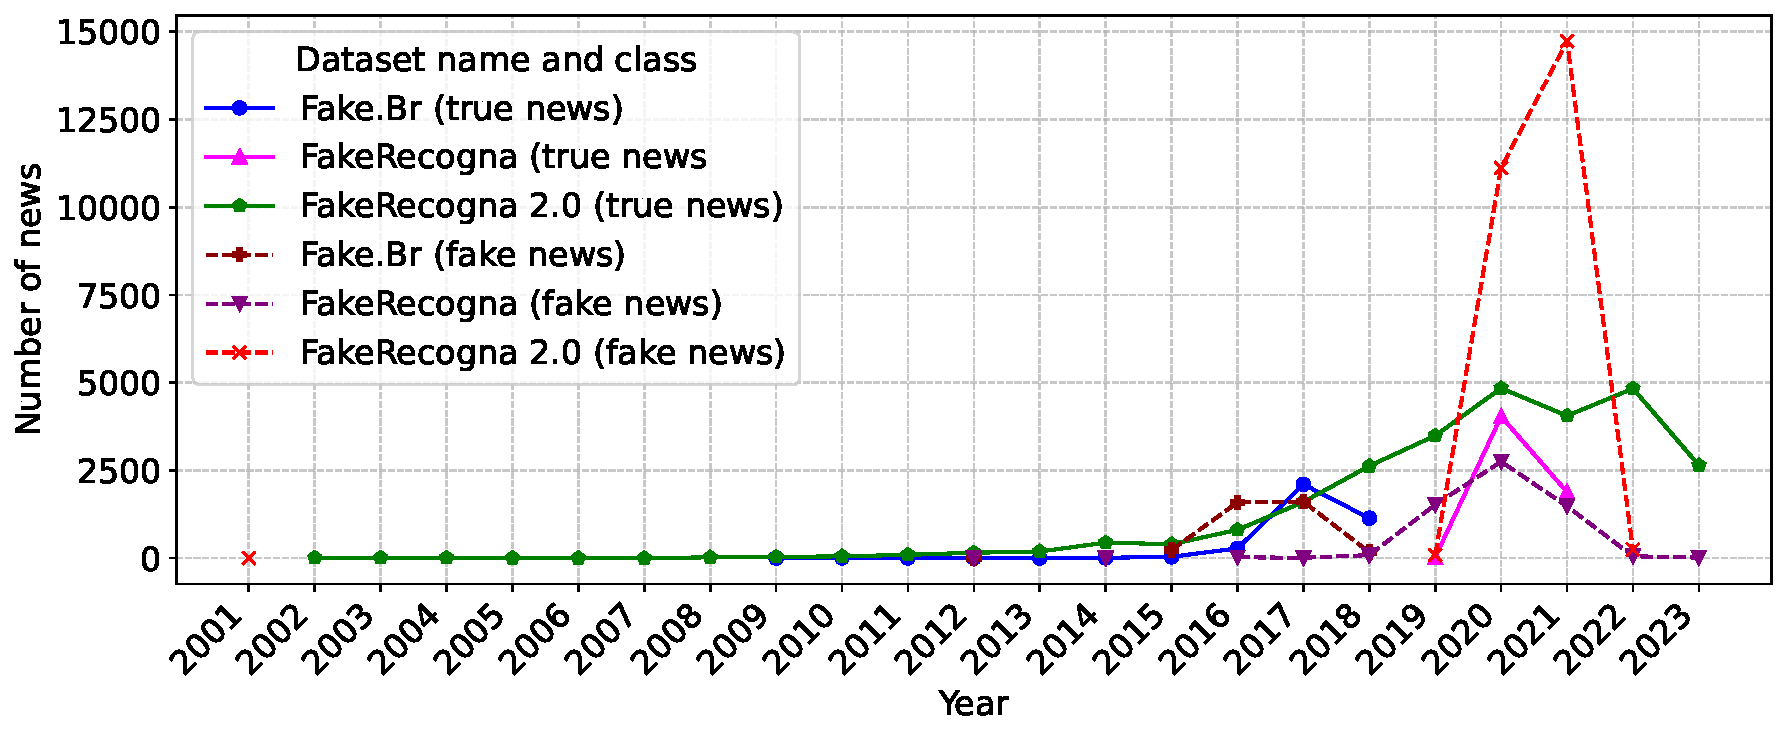
\includegraphics[width=\linewidth]{figs/archive/news_per_year.pdf}
%         \caption{Example left panel using a PDF plot.}
%         \label{fig:example_left}
%     \end{minipage}
%     \hfill
%     \begin{minipage}{0.48\linewidth}
%         \centering
%         % PNG is useful for raster images and screenshots.
%         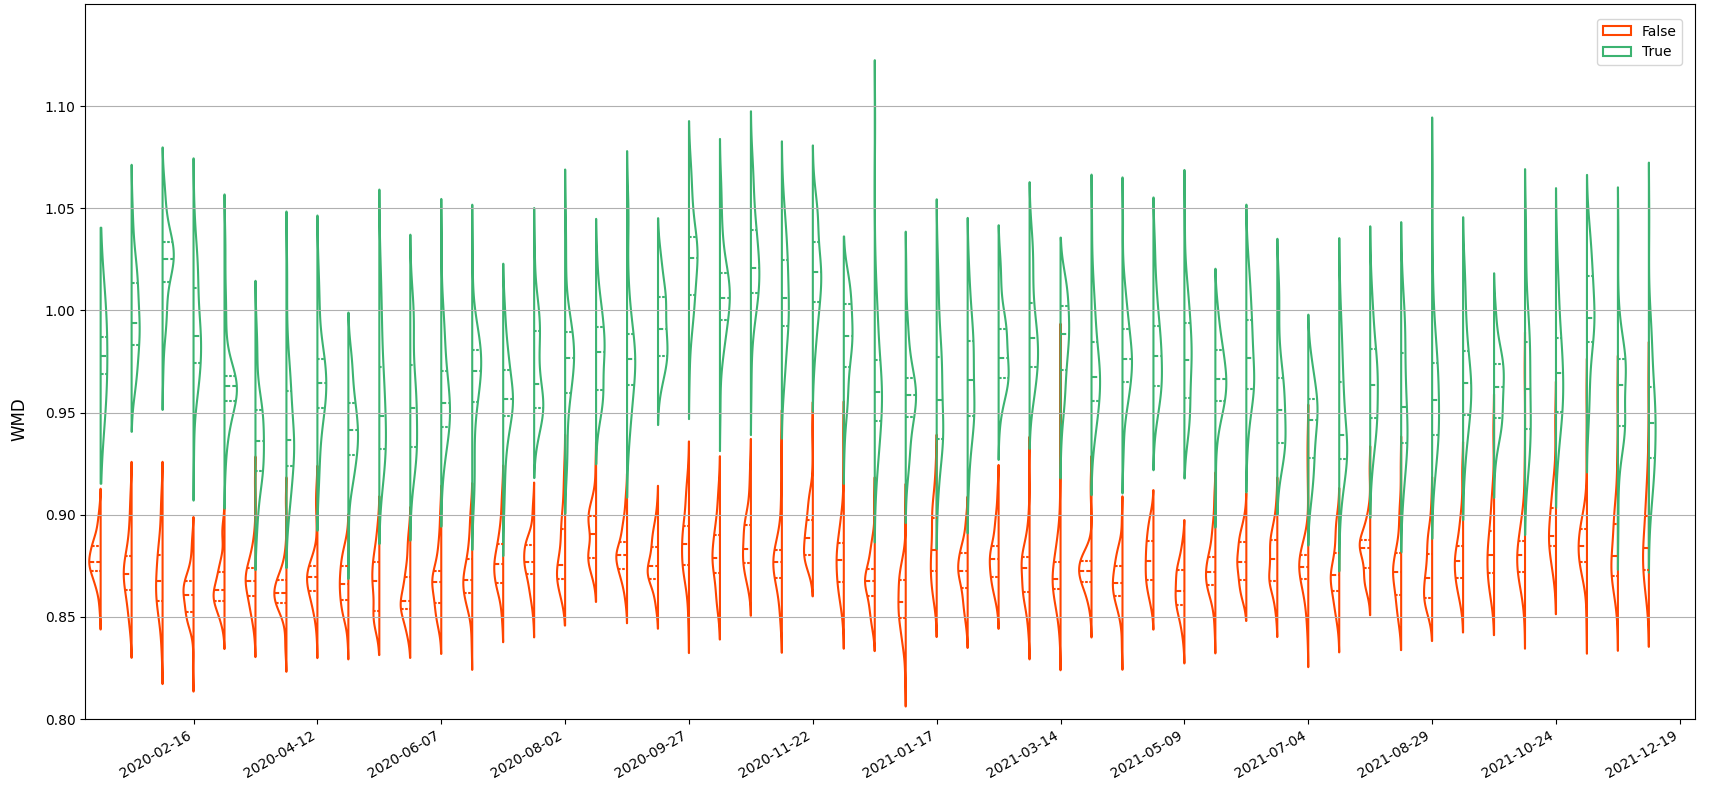
\includegraphics[width=\linewidth]{figs/archive/word_mover_distance_comparison_01.png}
%         \caption{Example right panel using a PNG image.}
%         \label{fig:example_right}
%     \end{minipage}
% \end{figure}
%
% If you want one caption for both images, use a single figure environment
% and write the shared caption after the two minipages.

% Example of table usage:
% \begin{table}[H]
%     \centering
%     \caption{Example table caption.}
%     \label{tab:example}
%     \begin{tabular}{lcc}
%         \toprule
%         Model / Setting & Value 1 & Value 2 \\
%         \midrule
%         Baseline & 0.00 & 0.00 \\
%         Proposed & 0.00 & 0.00 \\
%         \bottomrule
%     \end{tabular}
% \end{table}

% Example of a wider table with alignment:
% \begin{table*}[t]
%     \centering
%     \caption{Example of a wider comparison table.}
%     \label{tab:wide_example}
%     \begin{tabular}{lccc}
%         \toprule
%         Period & Documents & Drift score & Notes \\
%         \midrule
%         1986--1990 & 120 & 0.18 & Early period \\
%         1991--1995 & 145 & 0.27 & Transitional period \\
%         1996--2000 & 162 & 0.34 & Stronger semantic shift \\
%         \bottomrule
%     \end{tabular}
% \end{table*}

% Example of equation usage:
% \begin{equation}
%     d_t = 1 - \cos(\mathbf{x}_t, \mathbf{x}_{t-1})
% \end{equation}

% Example of referring to figures, tables, and sections in text:
% Figure~\ref{fig:cpd_example} illustrates the temporal pattern.
% Table~\ref{tab:example} summarizes the main results.
% Section~\ref{sec:methodology} details the experimental setup.

% Example of subsection usage:
% \subsection{Temporal aggregation}
% Describe how documents are grouped by month, quarter, year, or another unit.

% Example of itemized contributions:
% \begin{itemize}
%     \item We introduce a Portuguese temporal corpus for [task].
%     \item We compare [method A] and [method B].
%     \item We provide an analysis of [main finding].
% \end{itemize}

\end{document}
